\documentclass[letter,11pt]{article}

\usepackage{amsfonts}
\usepackage{amsmath}
\usepackage{amssymb}
\usepackage[brazilian]{babel}
\usepackage{enumerate}
\usepackage[T1]{fontenc}
%\usepackage[ansinew,latin1]{inputenc}
\usepackage[utf8x]{inputenc}
\usepackage{multicol}
\usepackage{graphicx}
\setlength\columnseprule{0.5pt}

\newtheorem{exer}{Exercício}
\newtheorem{teo}{Teorema}

\newcommand{\var}{Var}
\newcommand{\E}{\mathbb{E}}

\newcommand{\mat}[1]{\mbox{\boldmath{$#1$}}}

\usepackage[letterpaper,top=3cm, bottom=2cm, left=2.5cm, right=2.5cm]{geometry}

\begin{document}

%\thispagestyle{empty}
\begin{center}{ \Large MAT02023 - Inferência A }\end{center}

\begin{center}
{\large  \sc Gabarito Lista 7 - Consistência e Eficiência}
\end{center}
\vspace{5mm}

%%%%%%%%%%%%%%%%%%%%%%%%%%%%%%%%%%%%%%%%%%%%%%%%%%%%%%%%%%%%%%%%%%%%%%%%%%%%%%%%%%%%%
% Bolfarine e Sandoval - pg 30
\begin{exer} \rm
% Seja $X_1, \ldots, X_n$ uma amostra aleatória de $X \sim Poisson(\lambda)$. Considere que queremos estimar $\tau(\theta) = P(X=0) = e^{-\theta}$. Defina a estatística $S(\boldsymbol{X}) = \sum_{i=1}^n X_i$ e o estimador $W$ tal que
% \begin{equation}
% W(\boldsymbol{X}) = \left\{
% \begin{tabular}{c}
% 1, se $X_1 = 0$ ou \nonumber \\
% 0, caso contrário. \nonumber
% \end{tabular}
% \right.
% \end{equation}
% Encontre um estimador melhor do que $W$ baseado em $S$.
\end{exer}
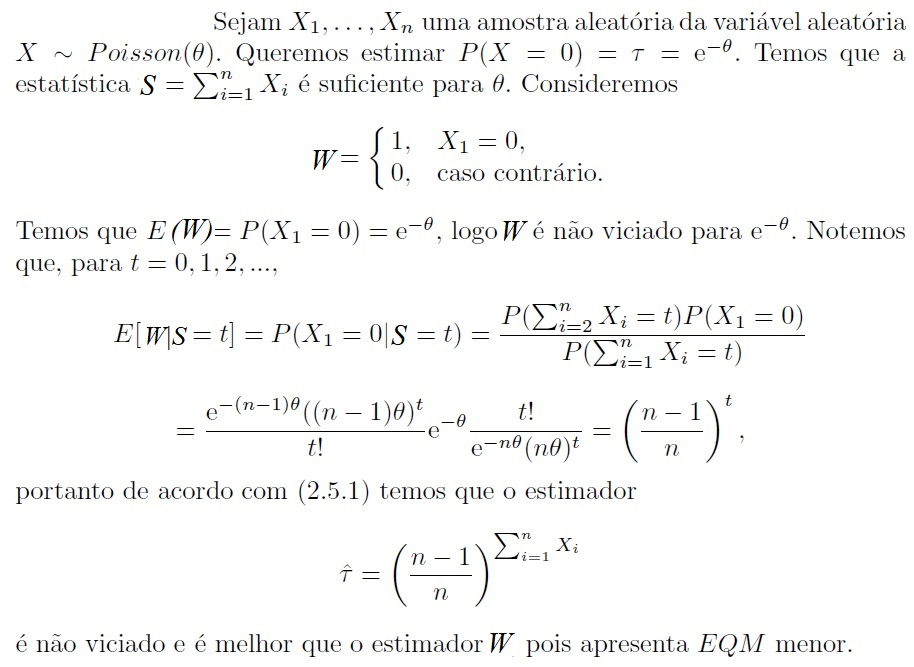
\includegraphics[scale=0.7]{gabarito_ex1_lista7.jpg}


% Notas de Aula, pg. 70
\begin{exer} \rm
% Prove o Teorema de Rao-Blackwell, que diz: se $W(\boldsymbol{X})$ é um estimador não viesado para $\tau(\theta)$, então $\widehat{\theta} = E \left( W \vert S\right)$ é não viesado para $\tau(\theta)$ e $Var ( \widehat{\theta} ) \leq Var \left( W \right)$.
Notas de Aula, pg. 70
\end{exer}


\begin{exer} \rm
% Para os dados do exercício 1 acima, utilize o teorema de Lehmann-Scheffé para mostrar que $\overline{X}$ é ENVVUM para $\lambda$.
\end{exer}


%(Teorema 10.1.3, Casella e Berger).
\begin{exer} \rm
% Prove que consistência forte de estimadores implica em consistência fraca. 
Demonstração da Proposição 2.2 (i) das 'Notas de Aula', pg. 74.
\end{exer}


% (Teorema 10.1.3, Casella e Berger).
\begin{exer} \rm
% Mostre que se $lim_{n \rightarrow \infty} Var \left[ W_n(\boldsymbol{X}) \right] = 0$ e $lim_{n \rightarrow \infty} \textit{Viés} \left[ W_n(\boldsymbol{X}) \right] = 0 \Rightarrow W_n(\boldsymbol{X})$ é consistente.
Demonstração da Proposição 2.2 (ii) das 'Notas de Aula', pg. 74.
\end{exer}

%%%%%%%%%%%%%%%%%%%%%%%%%%%%%%%%%%%%%%%%%%%%%%%%%%%%%%%%%%%%%%%%%%%%%%%%%%%%%%%%%%%%
\begin{exer} \rm
% Seja $X_1,X_2,\cdots,X_n$ uma amostra aleatória, onde $X_j\sim Uniforme(0,\theta)$, para todo $j=1,\cdots,n$, $\theta \in \Theta=(0,\infty)$.  %Rohatgi pagina 348
% \begin{enumerate}[a)]
%   \item Seja $X_{(n)} = \max(X_1,\cdots,X_n)$. Mostre que $X_{(n)}$ é um estimador consistente fraco para $\theta$;
%   \item Considere $Y_n=2\overline{X}$. Verifique se $Y_n$ é consistente para $\theta$.
% \end{enumerate}
???
\end{exer}

%%%%%%%%%%%%%%%%%%%%%%%%%%%%%%%%%%%%%%%%%%%%%%%%%%%%%%%%%%%%%%%%%%%%%%%%%%%%%%%%%%%%%
\begin{exer} \rm
% Seja $X_1,X_2,\cdots,X_n$ uma amostra aleatória, onde $X_j\sim Uniforme(0,\theta)$, para $j=1, \ldots, n$. Mostre que $W(\boldsymbol{X}) = \left(\prod_{j=1}^{n}X_j\right)^\frac{1}{n}$ é um estimador consistente para $\theta e^{-1}$. \\
% \noindent Dica: Use $W^\ast(\mat{X})=\log(W(\mat{X}))$ e a Lei Fraca dos Grandes Números. 
%Rohatgi pagina 348
\end{exer}


% \vspace{0.5cm}
%%%%%%%%%%%%%%%%%%%%%%%%%%%%%%%%%%%%%%%%%%%%%%%%%%%%%%%%%%%%%%%%%%%%%%%%%%%%%%%%%%%%
% lista 10 Paty - exercicios 4 e 5
\begin{exer} \rm
% Seja $X_1,X_2,\cdots,X_n$ uma amostra aleatória, onde $X_j$, para $j=1, \ldots, n$, possui função densidade de probabilidade dada pela expressão abaixo
% $$f_{X}(x)=(1-\theta)+\frac{\theta}{2\sqrt{x }}x^{\theta-1}I_{[0,1]}(x),$$
% \noindent onde $\theta\in[0,1]$.
% \begin{enumerate}[a)]
% \item Mostre que $\overline{X}$ é um, estimador viciado para $\theta$ e calcule o seu vício;
% \item Verifique se $\overline{X}$ é um estimador assintoticamente não viciado para $\theta$;
% \item Verique se $\overline{X}$ é um estimador consistente para $\theta$.
% \end{enumerate}
\end{exer}
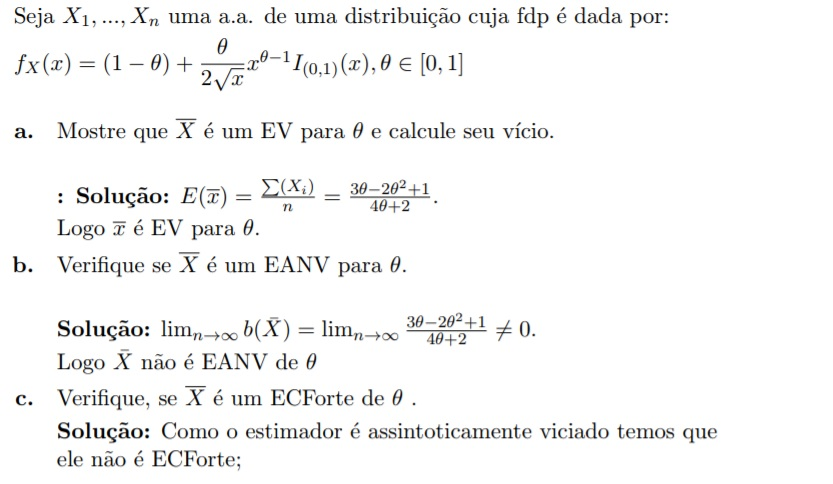
\includegraphics[scale=0.7]{gabarito_ex8_lista7.jpg}


\begin{exer} \rm
% Seja $X_1, X_2, \ldots, X_n$ uma amostra aleatória, onde $E(X_j) = \mu$ e $Var(X_j) = \sigma^2$, para todo $j=1, \ldots, n$, $\sigma^2$ finita. Verifique se  $\overline{X}$ and $S^2$ são estimadores consistentes de, respectivamente, $\mu$ e $\sigma^2$. \\
% \noindent Dica: Seja $X_1,X_2,\cdots,X_n$ é uma a.a., onde cada $X_j$ possui função densidade de probabilidade $f_X(\cdot)$  e $\E|X_j|^p<\infty$, para algum inteiro positivo $p$ e $j=1,\cdots,n$. Então, para $1\leqslant k\leqslant p$,
% $$\frac{1}{n}\sum_{j=1}^{n}X_j^k\longrightarrow^{\hspace{-.5cm}\prob}\hspace{.4cm} \E(X^k).$$
\end{exer}
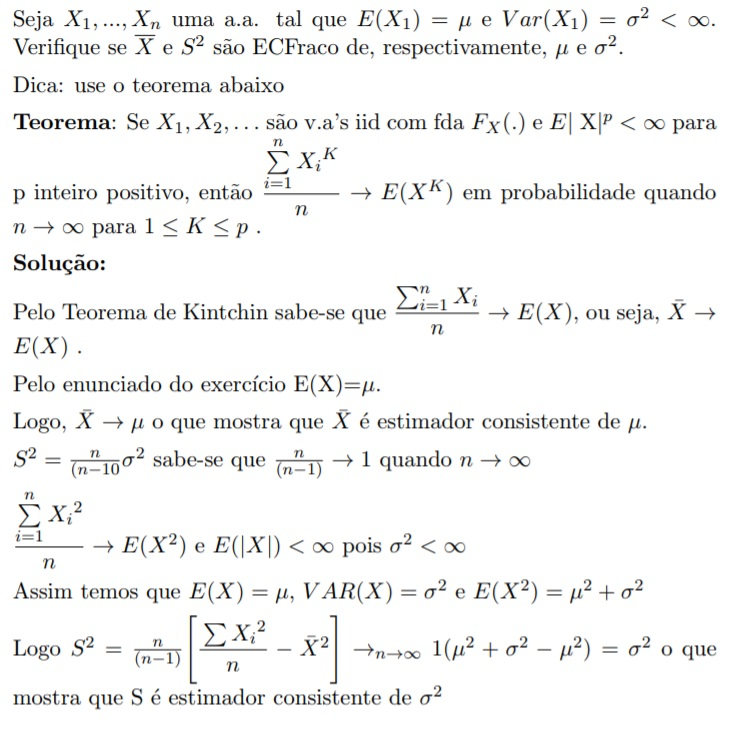
\includegraphics[scale=0.7]{gabarito_ex9_lista7.jpg}

%%%%%%%%%%%%%%%%%%%%%%%%%%%%%%%%%%%%%%%%%%%%%%%%%%%%%%%%%%%%%%%%%%%%%%%%%%%%%%%%%%%%
% Questões Markus

\begin{exer} \rm
% Explique o significado de:
% \begin{enumerate}[a)]
%   \item Viés, ou vício de um estimador;
%   \item Eficiência;
%   \item ENVVUM;
%   \item Desigualdade de Crámer-Rao;
%   \item Consistência forte;
%   \item Consistência fraca;
%   \item Estimador assintóticamente não viesado;
%   \item Eficiência assintótica;
% \end{enumerate}
\end{exer}


\begin{exer} \rm
% Comente o que significa, para a inferência pontual, o teorema de Rao-Blacwell.
\end{exer}


\begin{exer} \rm
% Qual a utilidade do Teorema de Lehmann-Scheffé?
\end{exer}

%%%%%%%%%%%%%%%%%%%%%%%%%%%%%%%%%%%%%%%%%%%%%%%%%%%%%%%%%%%%%%%%%%%%%%%%%%%%%%%%%%%%
% lista 9 Marcia
\begin{exer} \rm
% Suponha que $X_1; \ldots, X_n$ é uma amostra aleatória da distribuição Normal com média desconhecida $\theta \neq 0$ e variância conhecida $\sigma^2$. Utilize o Método Delta para determinar a distribuição assintótica de $\overline{X}^3$.
\end{exer}
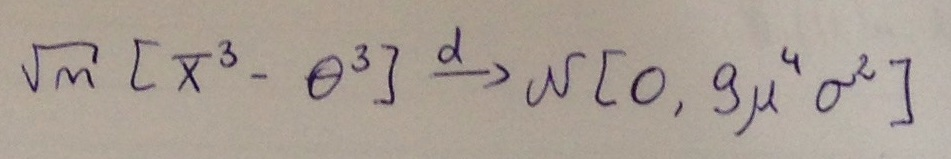
\includegraphics[scale=0.3]{gabarito_ex13_lista7.jpg}



\begin{exer} \rm
% Suponha que $X_1, \ldots, X_n$ é uma amostra aleatória da distribuição Exponencial com parâmetro $\beta$. A densidade de probabilidade é dada por $f(x|\beta) = \beta\exp\{-\beta x\}I_{(0,\infty)}(x)$,
% \begin{enumerate}[a)]
%   \item Encontre $\hat{\beta}_n$, o estimador de máxima verossimilhança para $\beta$.
%   \item Se $n$ é grande, a distribuição de $\hat{\beta}_n$ será aproximadamente Normal com média $\beta$. Mostre que a variância desta distribuição Normal será $\beta^2/n$.
%   \item Use o Método Delta para encontrar a distribuição assintótica de $1/\hat{\beta}_n$.
%   \item Mostre que $1/\hat{\beta}_n=\overline{X}$ e utilize o Teorema Central do Limite para determinar a distribuição assintótica de $\hat{\beta}_n$.
% \end{enumerate}
\end{exer}
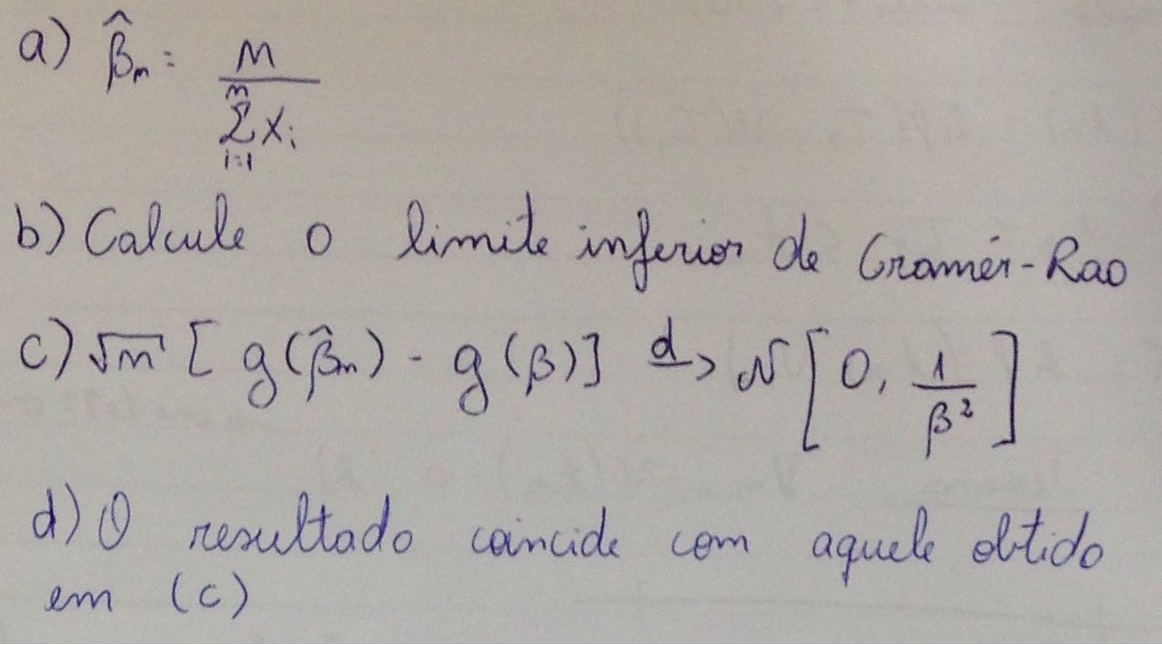
\includegraphics[scale=0.4]{gabarito_ex14_lista7.jpg}


\begin{exer} \rm
% Seja $Y_n$ uma variável aleatória com distribuição $\chi^2_n$. É possível mostrar que quando o tamanho amostral $n$ é grande, a formulação $(Y_n-n)/\sqrt{2n}$ terá aproximadamente distribuição Normal (0,1).
% \begin{enumerate}[a)]
%   \item Mostre que $\frac{(Y_n-n)}{\sqrt{2n}}=\sqrt{n}\left(\frac{Y_n}{n\sqrt{2}}-\frac{1}{\sqrt{2}} \right)$.
%   \item Considere o estimador $W_n(X) = \frac{Y_n}{n\sqrt{2}}$. Qual a distribuição assintótica de $W_n$.
%   \item Considere a função $g(u)=\sqrt{u}$, consequentemente $g'(u)=1/2\sqrt{u}$. Determine a distribuição assintótica de $g[W_n(X)]$.
% \end{enumerate}
\end{exer}
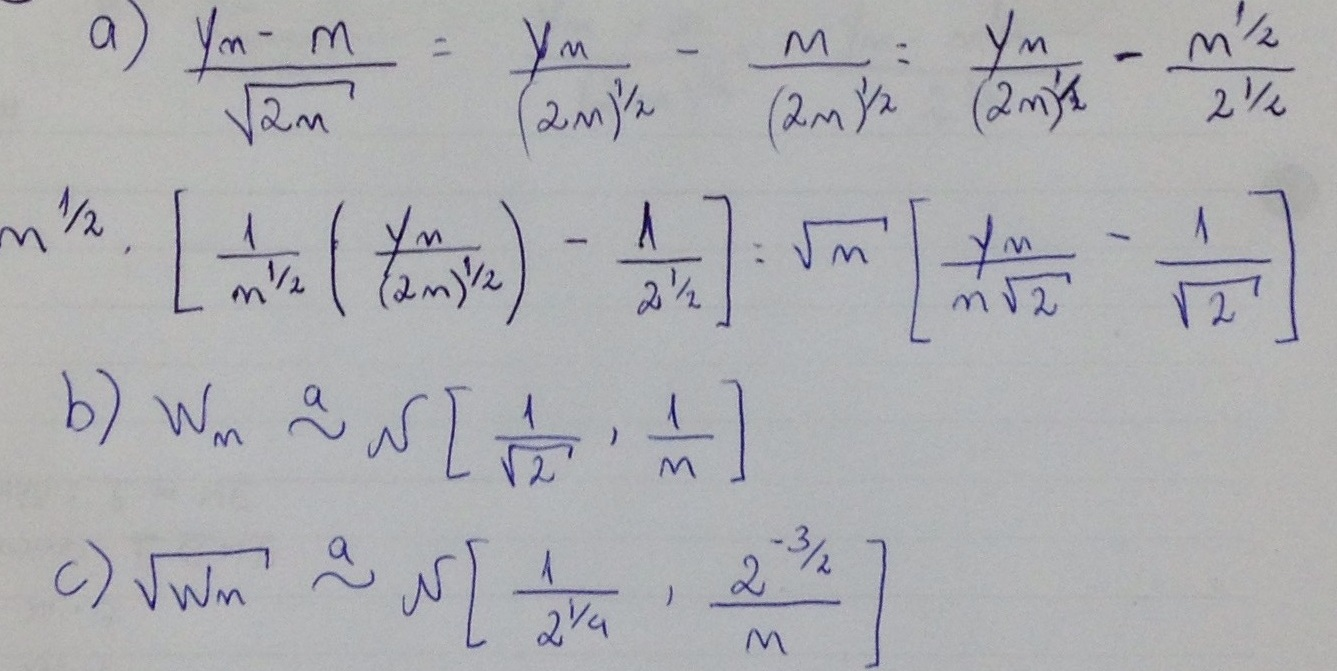
\includegraphics[scale=0.4]{gabarito_ex15_lista7.jpg}


\begin{exer} \rm
% Seja $Y_n$ uma variável aleatória com distribuição Poisson$(n)$. Para uma amostra grande, temos que a distribuição de $(Y_n -n)/\sqrt{n}$ será aproximadamente $N(0, 1)$. Considere a função $g(u) = u^2$.
% Obtenha a distribuição assintótica de $g(Y_n/n)$. \\
% \noindent Dica: Considere resultados similares ao que foi feito nos itens (a) e (b) da Questão 14.
\end{exer}
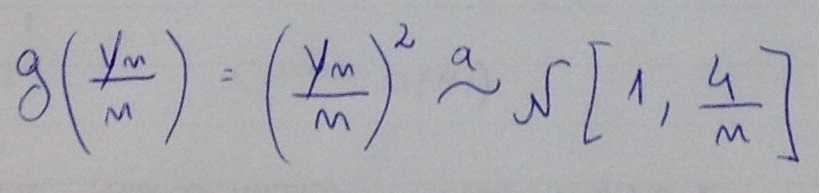
\includegraphics[scale=0.4]{gabarito_ex16_lista7.jpg}


\begin{exer} \rm
% Qual a diferença entre a Informação de Fisher Observada e a Esperada?
\end{exer}
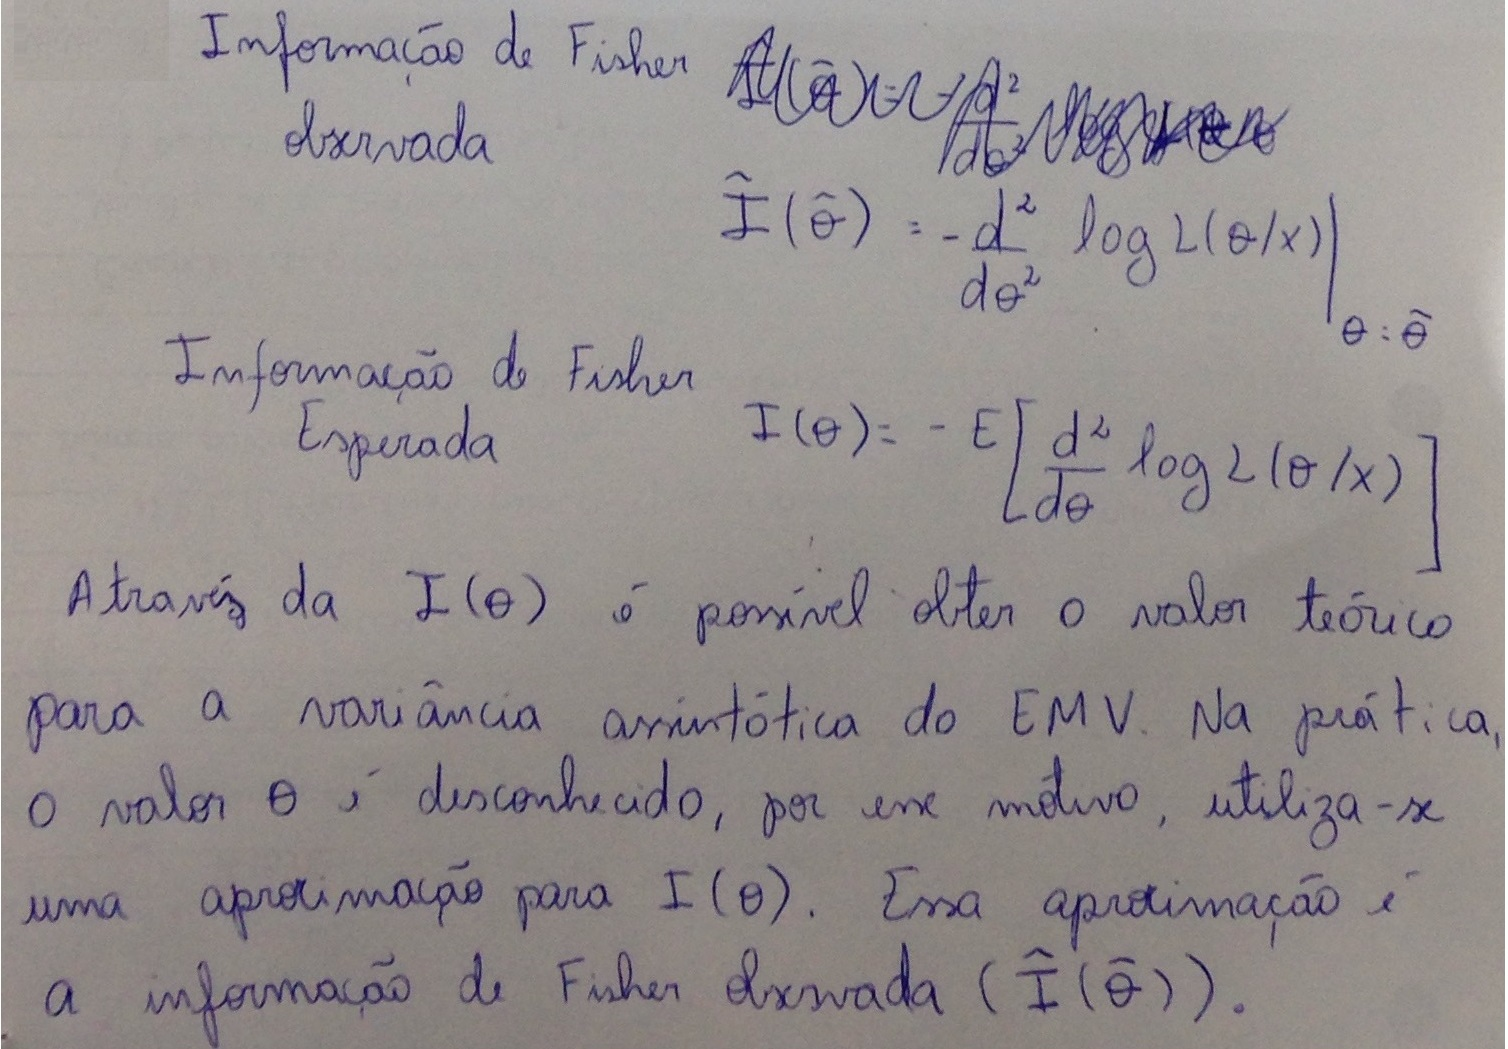
\includegraphics[scale=0.4]{gabarito_ex17_lista7.jpg}


% QUestao Markus?
\begin{exer} \rm
% Indique o enunciado do Teorema de Lehmann–Scheffé. Comente sobre as suposições e resultados.
???
\end{exer}

\end{document}